%-----------------------------------------------------------------------------
%	 Internet de las Cosas
%-----------------------------------------------------------------------------

\lhead[\thepage]{Internet de las Cosas \thechapter. \rightmark}
\rhead[Internet de las Cosas \thechapter. \leftmark]{\thepage}

%	Capitulo N: Internet de las Cosas
\chapter{Internet de las Cosas}
\markboth{Internet de las Cosas}{Internet de las Cosas}
\section{Definición}
El ``Internet de las Cosas", también conocido como IoT por sus siglas en inglés es el término utilizado para designar al conjunto de artefactos y dispositivos que poseen la capacidad de conectarse entre ellos o a otras redes como el internet de forma que pueden transmitir y recibir datos e información. De manera formal no existe una definición estandarizada sobre el concepto de IoT, pues dependiendo de la organización puede considerarse el concepto desde el punto de vista desde el cual se observe el concepto, sea desde la perspectiva de las redes, desde el punto de vista de los dispositivos o bien desde el punto de vista de los sistemas automatizados.\\

La primera aparición del término fue realizada en la conferencia ``Congressional Black Caucus Foundation 15th Annual Legislative Weekend'' en Washington, D. C. en septiembre del año 1985 por parte de Peter Lewis \cite{IoTTrueHistory} en donde define que ``El Internet de las cosas, o IoT, es la integración de personas, procesos y tecnología con dispositivos y sensores conectables para permitir el monitoreo, estado, manipulación y evaluación remota de las tendencias de dichos dispositivos''\cite{IoTFirstDef}.\\

Sin embargo este concepto fue olvidado hasta el año 1999 cuando Kevin Ashton independientemente lo utilizó ilustrar el poder de conectar Etiquetas de Identificación por Radio Frecuencia (RFID) usadas en las cadenas de suministro corporativas a Internet para contar y rastrear mercancías sin la necesidad de intervención humana\cite{iotInternetSociety}.\\

Para fines prácticos, durante esta investigación se toma el concepto de original de Peter Lewis, al ser una propuesta genérica e independiente del aspecto funcional examinado. Sin embargo es importante recalcar el hecho que las Las diversas definiciones de IoT no necesariamente están en desacuerdo, sino que enfatizan diferentes aspectos de las tecnologías aplicadas sobre los dispositivos IoT desde diferentes puntos focales y casos de uso. \cite{iotInternetSociety}

\vspace{50px}

\section{Modelos de Comunicación}
Desde el punto de vista teórico, los dispositivos IoT pueden interconectarse de varias formas. Estos siguen el marco de desarrollo planteado por el estandar RFC-7452\cite{rfc7452} en el que se plantean 4 modelos de comunicación con características propias. Esos modelos son:

\subsection{Comunicación Dispositivo a Dispositivo}
Este modelo de comunicación es el mas simple de todos los paradigmas y consiste básicamente en poder conectar directamente los dispositivos independientemente del medio usado Los dispositivos se comunican usando alguno de los protocolos y estándares disponibles que sean capaces de comprender. En el ámbito del IoT esta comunicación se realiza de manera inalambrica y donde los datos o instrucciones suelen ser bastante pequeños o poco frecuentes (figura \ref{fig:d2d}). En grandes cantidades estaríamos en presencia de un modelo netamente distribuido.
\begin{figure}[htb]
\centering
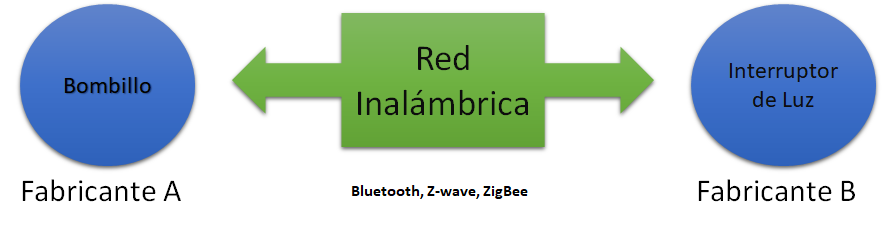
\includegraphics[scale=0.4]{./Figuras/d2d.png}
\caption{Modelo dispositivo a dispositivo}
\label{fig:d2d}
\end{figure}

  
\subsection{Comunicación Dispositivo a la Nube}
En el modelo de comunicación dispositivo a la nube, la conexión del dispositivo se conecta directamente a una nube (propia o federada) usando un proveedor de servicio (figura \ref{fig:d2n}). Este enfoque frecuentemente se aprovecha de los mecanismos de comunicación como redes celulares o la infraestructura de procesamiento de una  organización de manera directa para establecer la conexión entre el dispositivo y el servicio en la nube.
\begin{figure}[htb]
\centering
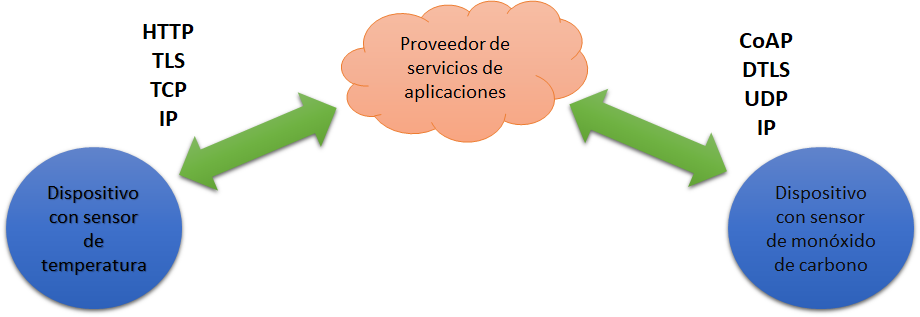
\includegraphics[scale=0.4]{./Figuras/d2n.png}
\caption{Modelo dispositivo a la nube}
\label{fig:d2n}
\end{figure}

\subsection{Comunicación Dispositivo a Puerta de Enlace}
El modelo de comunicación dispositivo a puerta de enlace establece una dispositivo o capa intermedia que concentre todas las comunicaciones (hub o broker) entre los dispositivos y de allí de ser necesario a otros fragmentos de la red o a internet (figura \ref{fig:d2g}). La ventaja de este enfoque es la capacidad de operar de manera centralizada parte de las comunicaciones de los dispositivos. Muchos protocolos están basados en el principio del paradigma de cliente-servidor por lo que este se adapta de manera natural al modelo.
\begin{figure}[htb]
\centering
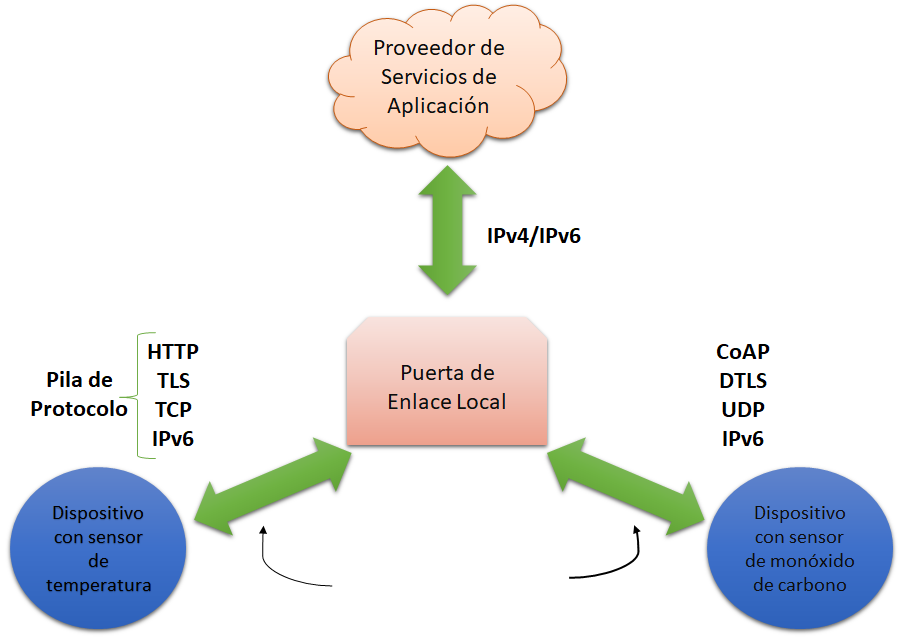
\includegraphics[scale=0.4]{./Figuras/d2g.png}
\caption{Modelo dispositivo a puerta de enlace}
\label{fig:d2g}
\end{figure}

\subsection{Comunicación Dispositivo a Intercambio de Datos en Back-end}
Este modelo es una forma automatizada de conexiones, en donde el dispositivo envía los datos a una o más APIs para de manera transparente, haciendo que este pueda intercambiar la información entre servicios que no necesariamente están estructurados o que pertenecen a un tercero (figura \ref{fig:d2b}). Particularmente este modelo es útil cuando se requiere que la información sea fácilmente accesible a través de múltiples plataformas o sistemas independientes.
\begin{figure}[htb]
\centering
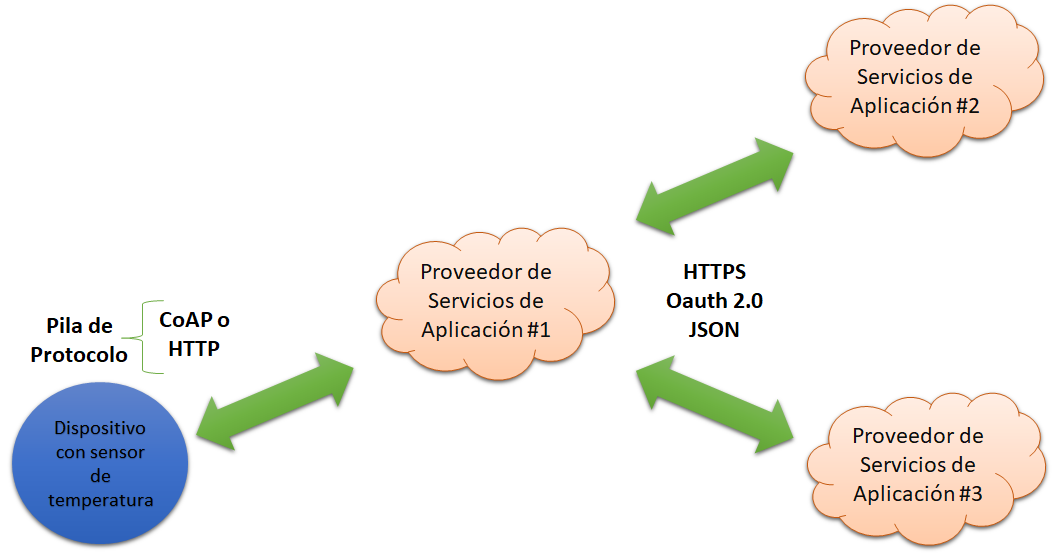
\includegraphics[scale=0.4]{./Figuras/d2b.png}
\caption{Modelo dispositivo a intercambio de datos en back-end}
\label{fig:d2b}
\end{figure}


\section{Aplicaciones del Internet de las Cosas}
hue
\subsection{Hogares}
hue
\subsection{Industrias}
hue
\subsection{Transporte y Logistica}
hue
\subsection{Comercio}
hue
\subsection{Tecnologías Vestibles}
hue
\subsection{Medicina y Salud}
hue
\subsection{Ciudades Inteligentes}
hue

\section{Interoperatividad entre Infraestructuras y Dispositivos}
hue
\subsection{Ecosistemas}
hue
\subsection{Restricciones}
hue
\subsection{Riesgos}
hue
\subsection{Sistemas Heredados}
hue
\subsection{Configuración de dispositivos}
hue

\section{Protocolos y Estándares Utilizados}
hue
\subsection{Protocolos}
hue
\subsubsection{HTTP}
hue
\subsubsection{MQTT}
hue
\subsubsection{IPv4 e IPv6}
hue
\subsection{Estándares}
hue
\subsubsection{Bluetooth}
hue
\subsubsection{Redes Celulares}
hue
\subsubsection{NFC}
hue
\subsubsection{Wifi}
hue
\subsubsection{Zigbee}
hue
\subsubsection{Z-Wave}
hue

\section{Seguridad}
hue.
